
\subsection{Datasets}  

\subsubsection{4-2-4 Encoder} 

TODO: Write it as "Because BAL had significantly worse performance on this experiment we tried to analyse what are the reasons and propose improvements". 

To compare the performance of BAL with GeneRec, we ran tests using the well-
known 4-2-4 encoder task, following O’Reilly \citet{o1996bio}. We investigated the convergence
of BAL and the number of required training epochs as a function of the learning
rate. Fig. 1 shows the convergence success for 100 networks and the average
numbers of epochs needed. The simulations showed that convergence of BAL
depends on the learning rate, with the highest number of 65\% successful runs
achieved for $\lambda = 0.9$ \citet{farkas2013bal}. For comparison, O’Reilly \citet{o1996bio} reports 90\% success for basic GeneRec algorithm and 56\% for a symmetric modification of GeneRec and its
modification equivalent to CHL. In sum, probability of BAL convergence is lower
than that of basic GeneRec rule, but comparable to its symmetric versions. We
expect that the smaller number of successful runs is in both cases influenced by
the bidirectional nature of the weight update.

\subsubsection{Complex Binary Vector Associations} 

TODO: Write it as "Small scale graphical task to see the reconstruction" 
We evaluated the network performance on n–to–1 data associations, motivated
by the sensory-motor mappings between distributed patterns. For this purpose
we created low-dimensional sparse binary codes, 16-dimensional vectors ($4 \times 4$
map) with k = 3 active units with n = 4. For each target (y), these four
patterns (x) were assumed to have nonzero overlap. Again, we searched for
optimal $\lambda$ and $n_H$ (Fig. 5). The best performance was achieved using $\lambda$ $\approx$ 1. We
can observe that the ambiguity in the data association causes the network to
produce errors in B direction. For the best $\lambda$ the networks yielded patSuccB $\approx$
4\% and $bitSucc^B \approx 86\%$, which means that the networks made small errors in
most patterns. This could be expected since the network cannot know which of
the four (x) patterns is to be reconstructed. It is known, that a network trained
to associate more binary target patterns with one pattern tends to produce a
mesh of outputs, weighed by their frequency of occurrence in the training set.
Examples of network outputs are illustrated in Fig. 6.

\begin{center} 
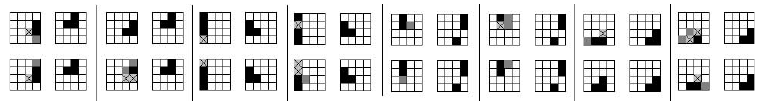
\includegraphics[width=0.8\textwidth]{img/cbva_back_repre.png} \citep{farkas2013bal}
\end{center} 

\subsubsection{Hand-written Digits} 
TODO: Write overview as "High dimensional graphical task to see backward representation and compare it with a bunch of other models" 
TODO: Compare results: \url{http://yann.lecun.com/exdb/mnist/} 
Data from MNIST database \citet{lecun1998gradient}. 

TODO: Dataset motivation: See blend and how performs on non-bijective functions. 

